\section{Data}
<<<<<<< HEAD
\section{Snell's Law}
\subsection{Air to Glass}

\subsection{Glass to Air}

\begin{figure}[h]
    \centering
    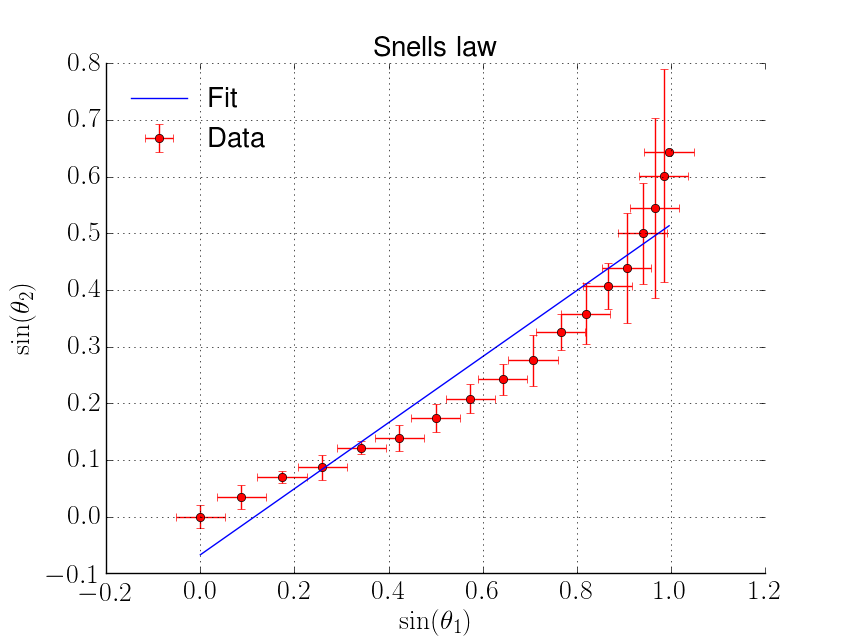
\includegraphics[width=0.5\textwidth]{snell}
    \caption{Dat\ldots}
    \label{fig:fit}
\end{figure}

\section{Reflection}
\subsection{p-polarized}
\subsection{s-polarized}
\begin{figure}[h]
    \centering
    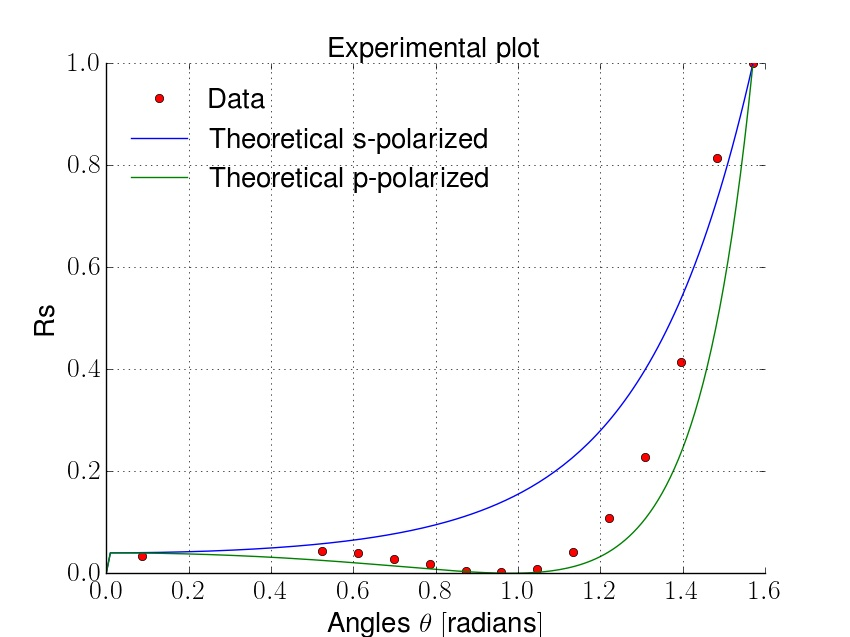
\includegraphics[width=0.5\textwidth]{reflection}
    \caption{Dat\ldots}
    \label{fig:reflection}
\end{figure}



\section{Transmission}
\subsection{p-polarized}
\subsection{s-polarized}
\begin{figure}[h]
    \centering
    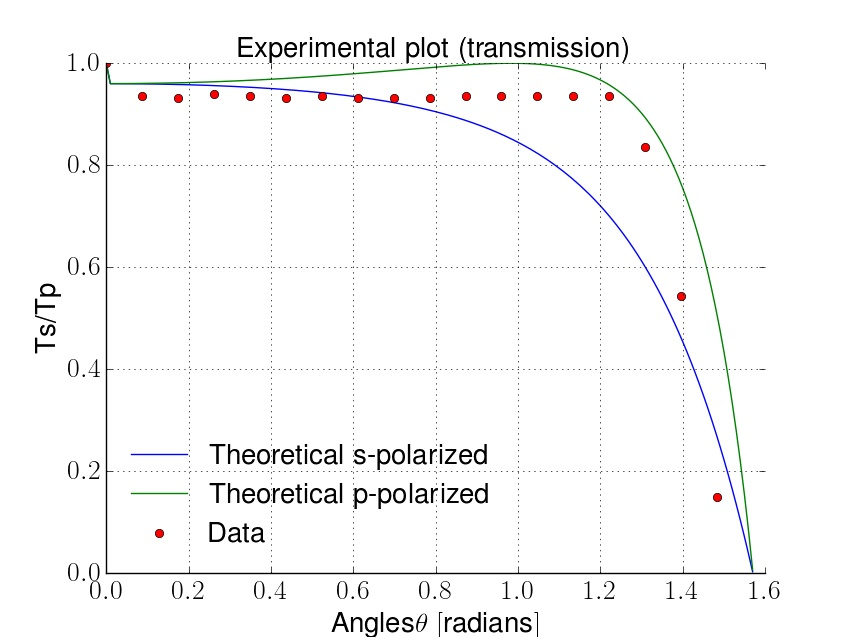
\includegraphics[width=0.5\textwidth]{transmission}
    \caption{Dat\ldots}
    \label{fig:transmission}
\end{figure}
=======
>>>>>>> 1545327077b28dc942b3bb9206f32173eec70362

\subsection{Snells law}

To determine our refractive index of the glass $n_2$we have used a linear fit between $\sin(\theta_1)$ - our incoming angle - and $\sin(\theta_2)$, where $\theta_2$ denotes our reflected angle. According to snells law the correlation between these quantities are:

\begin{align}
\frac{n_1}{n_2}\sin(\theta_1)=\sin(\theta_2)
\end{align}

since the refractive index of air is $n_1 \approx 1$ we can determine $n_2$ from our data as:

\begin{align}
n_2=\frac{1}{a}
\end{align}

where $a$ is the slope of a linear fit on our data. \\

On the plot we see our data and a linear fit to our data. One can clearly see that our data does not fit a linear tendency, but forcing the linear fit we can compute the refractive index of our glass from the slope of the fit to $n_2=1.7$ wich is 0.2 from the theoretical reflective index of the glass of $1.5$. The difference is relatively great, but thos should not surprise us with our data. 

\subsection{Fresnel relations}

To compute our transmission and reflection coefficients we have used the relationsship between the measured angle and the maximal intensity of our laser (the measured intensity at 90 degrees for reflection and at 0 degrees for transmission). For any given angle we have:

\begin{align}
R_(s/p)(\theta)=\frac{I(\theta)}{I(90)} \quad T_(s/p)(\theta)=\frac{I(\theta)}{I(0)}
\end{align}

Where the background was substracted from the used intensities. 

\subsubsection{Air to glass}

For this situation we have data for the transmission of $s$- and $p$-polarized light, but only we only have data regarding the reflection for our $p$-polarized light. This is due to the fact that we overranged the laser in order to get a measureble signal at low angles for the $s$-polarized light, but unfortunately the intensity of the laser signal then became greater than the detectors limit of 5 V at larger angels, thus we were not able to measure our maximal intensity. We intended to measure the s-polarized reflection again but ran out of time.\\

Looking at our p-polarized reflection we observe that our data generally does not match with the theory, since the theoretical curve does not lie within the error of our data. The error is computed using error proporgation for an uncertainty of 2 degrees on the incoming angle. We can, however, recognize some of the proporties of the theory in our data, such as the low reflection index at small angles with an increase in the percentage of transmitted light at angles above 1.2 radians. Our data actually also seem to fit very well at small angles, it even seems to fit best around the Brewster angle at $56$ degrees. Looking at greater angles our data tends towards one faster than theoretically expected. 

For our transmission, we see that we had some measurement problems for small angles for our p-polarized light, because it seems that our intensity is almost constant for small angles but follows the theoretical values for greater angles. It it also peculiar that our error for the small angles are small, even though this where our data deviates the most from the theory. Again our errors were computed using the error proporgation law. For the $s$-polarization we observe a lot of dispertion of our data around our theoretical plot for the small angles, but we seem to be corresponding with when the proper errors are taking into consideration.

